
\section{La complétion semi-automatique}

\begin{frame}{Définition complétion semi-automatique}
	\begin{columns}
		\column{0.45\textwidth}
		
		\textbf{En quelques mots~:}
		\begin{itemize}
			\item Assistance
			\item Proposition des suggestions
			\item Choix final fait par l'utilisateur
		\end{itemize}
		\vfill	
		\textbf{Utilisé dans de nombreuses applications~:}
		\begin{itemize}
			\item Traitement de texte
			\item IDE
			\item Moteurs de recherche
			\item Assistance virtuelle
		\end{itemize}
		\column{0.55\textwidth}
		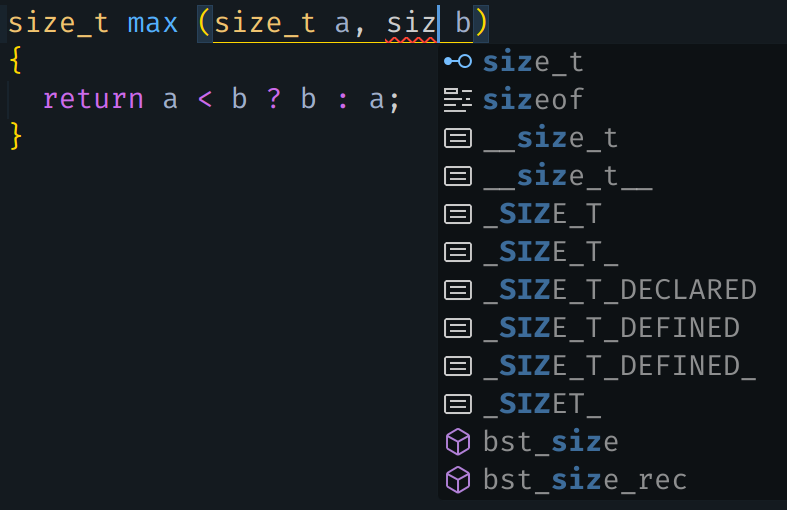
\includegraphics[width=\textwidth]{images/exemple_completion_semi_auto.png}
		\centering
		\uline{Exemple de complétion semi-automatique sur VS Code}
		
	\end{columns}
\end{frame}


\begin{frame}{Différence avec la complétion semi-automatique}
	\begin{columns}
		\column{0.48\textwidth}
		\textbf{Automatique}
		\begin{itemize}
			\item Pas besoin d'interaction manuelle
			\item Gain de temps maximal
			\item Peut générer des erreurs si le contexte est mal interprété
		\end{itemize}
		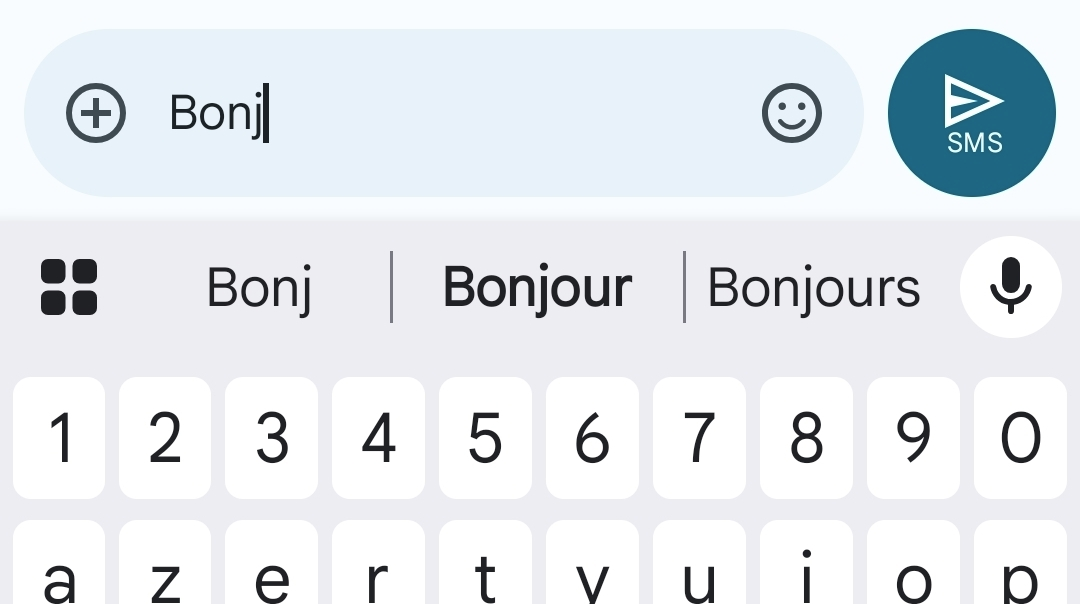
\includegraphics[width=0.9\textwidth]{images/exemple_clavier_completion_auto.png}
		
		\column{0.48\textwidth}
		\textbf{Semi-Automatique}
		\begin{itemize}
			\item Nécessite une validation manuelle
			\item Plus de contrôle pour l'utilisateur
			\item Moins d’erreurs
		\end{itemize}
		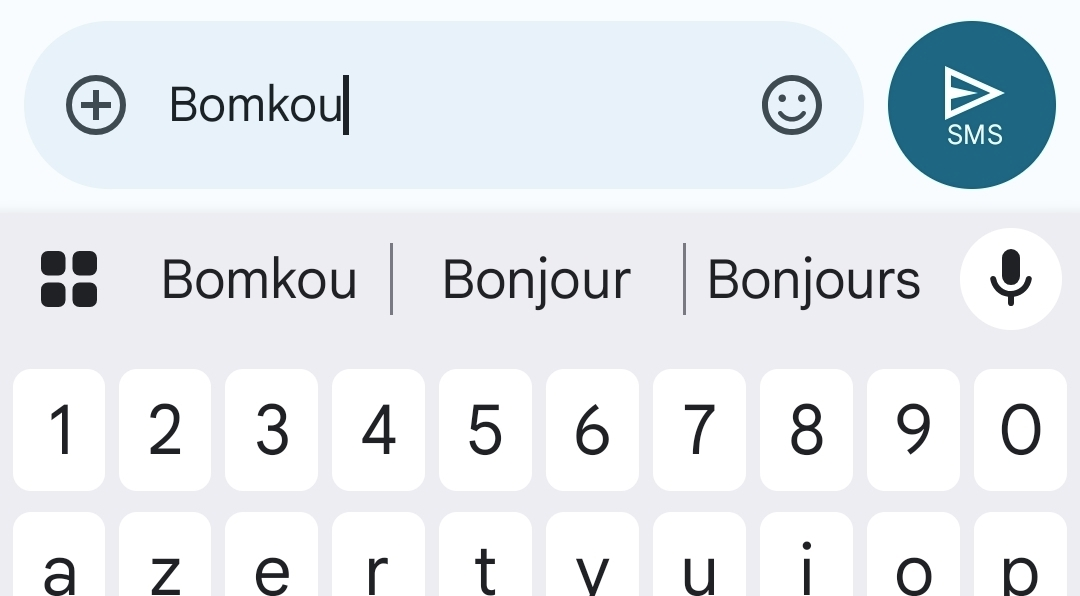
\includegraphics[width=0.9\textwidth]{images/exemple_clavier_completion_semi.png}
	\end{columns}
\end{frame}

% \begin{frame}{Cibest}
%     \begin{columns}[T]
%         \metroset{block=fill}
%         \column{0.45\textwidth}
%         \begin{exampleblock}{Cibest Solution}
%                 \textbf{Champs d'action~:}
%                 \begin{itemize}
%                     \item Domaine du logiciel\\embarqué
%                     \item Vidéoprotection
%                     \item Wifi passagers
%                     \item Comptage passagers
%                     \item Rétrovision numérique
%                 \end{itemize}

%                 \textbf{Statistiques~:}
%                 \begin{itemize}
%                     \item + de 450 clients équipés
%                     \item + de 200 villes en France
%                 \end{itemize}
%           \end{exampleblock}

%         \column{0.45\textwidth}
%         \begin{alertblock}{Cibest IT}
%             \textbf{Champs d'action~:}
%             \begin{itemize}
%                 \item Informatique dans les\\transports
%                 \item Billetique
%             \end{itemize}

%             \textbf{Statistiques~:}
%             \begin{itemize}
%                 \item + de 30 consultants clients équipés
%                 \item + de 200 villes en France
%             \end{itemize}
%           \end{alertblock}
%     \end{columns}
%     \end{frame}


%
% \section{Missions du Stage}
% \begin{frame}{Contexte et Problématique Actuelle}
% 	\begin{columns}
% 		\column{0.5\textwidth}
% 		\textbf{Contexte}
% 		\begin{itemize}
% 			\item Installation d'équipements
% 			\item Configurations personnalisées
% 			\item Sauvegarde des configurations
% 			\item Identification des problèmes
% 		\end{itemize}
% 		
% 		\column{0.5\textwidth}
% 		\textbf{Problématique}
% 		\begin{itemize}
% 			\item Récupération manuelle
% 			\item Perte de temps, erreurs
% 			\item Résultats sous diverses formes
% 			\item Absence de contrôle qualité
% 		\end{itemize}
% 	\end{columns}
% 	\vfill
% 	\centering\includegraphics[width=0.9\textwidth]{images/camera_bus.png}
% \end{frame}
%
% % Diapositive 2 : Besoins et Solution Proposée
% \begin{frame}{Besoins Identifiés et Solution Proposée}
% 	\begin{columns}
% 		\column{0.7\textwidth}
% 		\hspace*{-0.1\textwidth}
% 		\includegraphics[width=1.1\textwidth]{images/besoins_stage.pdf}
% 		\column{0.3\textwidth}
% 		\hspace*{-0.23\textwidth}
% 		\includegraphics[width=1.4\textwidth]{images/solution_stage.pdf}
% 	\end{columns}
% \end{frame}
% % Diapositive 2 : Besoins et Solution Proposée
% \begin{frame}{Besoins Identifiés et Solution Proposée}
% 	\begin{columns}
% 		\column{0.3\textwidth}
% 		\hspace*{-0.13\textwidth}
% 		\includegraphics[width=1.2\textwidth]{images/besoins_stage.pdf}
% 		
% 		\column{0.8\textwidth}
% 		
% 		\hspace*{-0.75cm}
% 		\includegraphics[width=1.125\textwidth]{images/solution_stage.pdf}
% 		
% 	\end{columns}
% \end{frame}
%
%
% \begin{frame}{Méthodologie de Travail}
% 	\begin{columns}[t]
% 		\column{0.5\textwidth}
% 		\textbf{Méthode Agile~:}\\[0.4cm]
% 		\hspace*{-0.4cm}
% 		\vspace*{-1cm}
% 		\begin{itemize}
% 			\item flexibilité
% 			\item adaptabilité
% 			\item amélioration continue
% 		\end{itemize}
% 		\includegraphics[width=1.1\textwidth]{images/schema_conception.png}
% 		\column{0.5\textwidth}
% 		\textbf{Outils Utilisés~:}
% 		\hspace*{0.2cm}
% 		\includegraphics[width=0.8\textwidth]{images/logo_outils.png}
% 	\end{columns}
% \end{frame}
